\section*{Assignment 02: Network Effects and Launch Strategy}
\addcontentsline{toc}{section}{Assignment 02: Network Effects and Launch Strategy}

\subsection*{How we engineered the loops}
SkillSync only works if students and organisations keep nudging each other, so we mapped the network effects explicitly. The cross-side loop is obvious: vetted NGO projects attract students, and their turnout convinces resource-strapped organisations to post again. On top sit two supportive loops: a student same-side effect driven by peer stories and cohort rituals \citep{Choudary2016}; and a data loop where each completed match enriches our skill taxonomy and matching algorithm, nudging us toward the curated-orchestrator archetype from \citet{Reillier2017}. It is a technical mapping of incentives and friction points, and it kept our debates grounded. Figure~\ref{fig:application-flow} shows one student journey traveling through these loops in under ten minutes.

\subsection*{Breaking the penguin problem}
The penguin problem hit us hard: no student wants to join before credible projects show up, yet NGOs hesitate without proven talent. First, we partnered with two anchor NGOs who already mentored students informally, securing the social proof \citet{HagiuWright2013} say you need. Second, we recruited a ``founding cohort'' of 40 students via faculty recommendations, course mailing lists, and targeted classroom visits, giving them concierge onboarding, stipends, and a moderated Slack space. Third, we launched projects with pre-filled briefs and promised replacement support if a match fizzled. The subsidies mirror playbooks from \citet{Gunasilan2024} and \citet{FarrellSaloner1986} and follow Lecture~4's guidance on solving the chicken-and-egg problem \citep{Lecture04}.

\subsection*{Launch strategy reflections}
Looking back, our soft launch favoured breadth over intensity. We opened the waitlist broadly and then scrambled to curate projects, which diluted the sense of community. If we reran it, I would narrow the first wave to one faculty and three NGOs with adjacent missions \citep{Choudary2016}, front-load measurement on time-to-first-value and project completion rate \citep{ShapiroVarian1999}, and invest earlier in student ambassadors because trusted peers beat email blasts.


\begin{figure}[H]
  \centering
  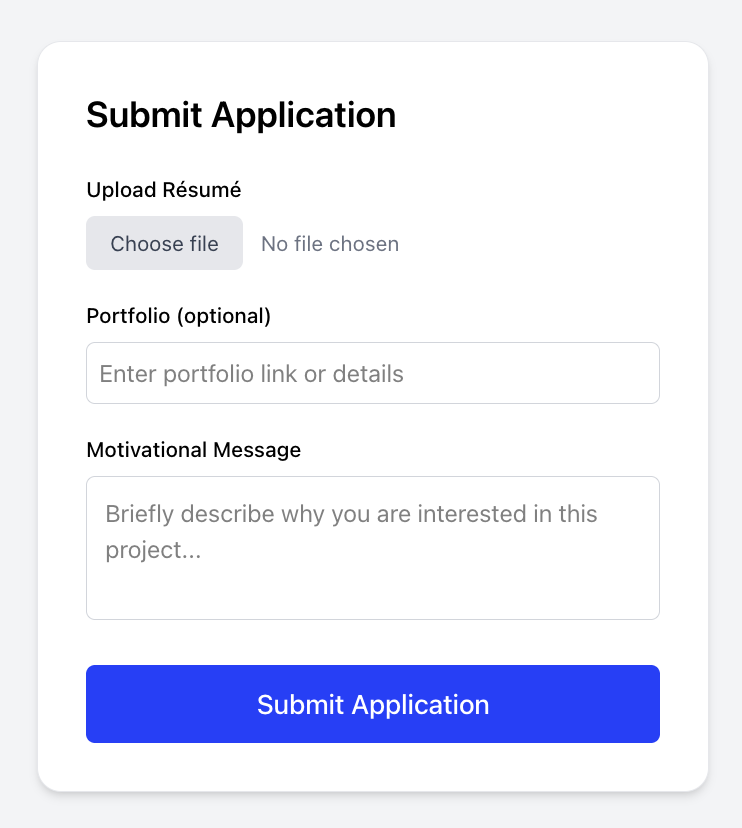
\includegraphics[width=0.85\linewidth]{Student-Submission.png}
  \caption{Student application flow with guided pitch submission.}
  \label{fig:application-flow}
\end{figure}

Figure~\ref{fig:application-flow} enforces discipline via sequenced prompts, live status, and scoped briefs.

We also revisited the organisational journey after the first dozen projects wrapped up. Figure~\ref{fig:project-creation} (in Assignment~3) shows the scoping prompts that keep briefs from arriving half-baked, and automations alert the founding cohort when new projects drop to keep acceptance under 24 hours.
